\documentclass[tikz,border=7pt]{standalone}
\usepackage{amsmath,amssymb}
\usepackage[scaled]{helvet}
\renewcommand{\familydefault}{\sfdefault}
\usetikzlibrary{arrows.meta,backgrounds,calc,fit,positioning,shapes.geometric}
\definecolor{bpink}{HTML}{172033}
\definecolor{bpblue}{HTML}{2A78D6}
\definecolor{bporange}{HTML}{E56A32}
\definecolor{bpgreen}{HTML}{168A65}
\definecolor{bppurple}{HTML}{7A5CC7}
\definecolor{bpred}{HTML}{C94A4A}
\definecolor{bpmuted}{HTML}{667085}
\definecolor{bpgrid}{HTML}{D8DEE8}
\definecolor{bpsurface}{HTML}{F8FAFC}
\tikzset{
  var/.style={circle,draw=bpblue,fill=bpblue!10,line width=.9pt,minimum size=8mm,font=\small\bfseries,text=bpink},
  factor/.style={rectangle,rounded corners=1.5pt,draw=bporange,fill=bporange!14,line width=.9pt,minimum size=6.8mm,font=\small\bfseries,text=bpink},
  constraint/.style={rectangle,rounded corners=1.5pt,draw=bpred,fill=bpred!12,line width=.9pt,minimum size=6.8mm,font=\small\bfseries,text=bpink},
  edge/.style={draw=bpmuted!75,line width=.9pt},
  msgvf/.style={-{Latex[length=2.2mm]},draw=bpblue,line width=1.35pt},
  msgfv/.style={-{Latex[length=2.2mm]},draw=bporange,line width=1.35pt},
  label/.style={font=\scriptsize,text=bpmuted,align=center},
  title/.style={font=\bfseries\large,text=bpink},
  card/.style={draw=bpgrid,fill=bpsurface,rounded corners=7pt,line width=.7pt},
}

\begin{document}
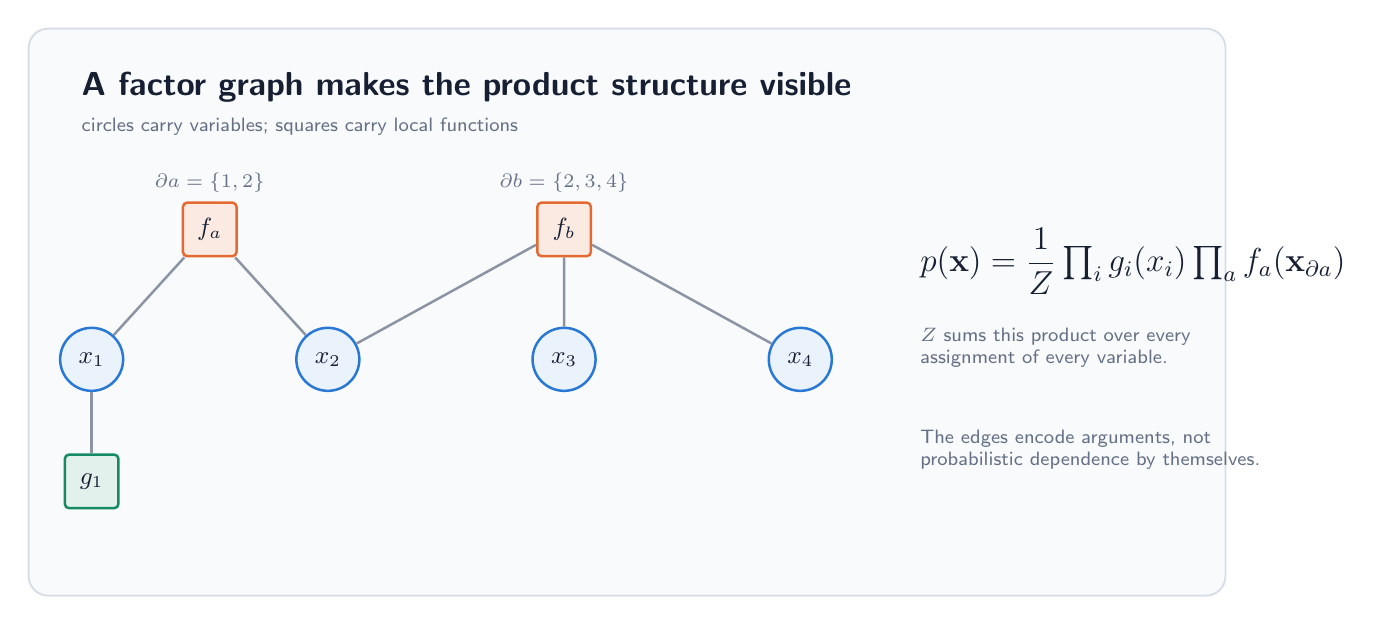
\begin{tikzpicture}[font=\sffamily]
  \node[card,minimum width=15.2cm,minimum height=7.2cm] at (6.8,2.4) {};
  \node[title,anchor=west] at (-.25,5.25) {A factor graph makes the product structure visible};
  \node[label,anchor=west] at (-.25,4.75) {circles carry variables; squares carry local functions};
  \node[var] (x1) at (0,1.8) {$x_1$};
  \node[var] (x2) at (3,1.8) {$x_2$};
  \node[var] (x3) at (6,1.8) {$x_3$};
  \node[var] (x4) at (9,1.8) {$x_4$};
  \node[factor] (a) at (1.5,3.45) {$f_a$};
  \node[factor] (b) at (6,3.45) {$f_b$};
  \node[factor,draw=bpgreen,fill=bpgreen!12] (g) at (0,.25) {$g_1$};
  \draw[edge] (g)--(x1);
  \draw[edge] (a)--(x1) (a)--(x2);
  \draw[edge] (b)--(x2) (b)--(x3) (b)--(x4);
  \node[label] at (1.5,4.05) {$\partial a=\{1,2\}$};
  \node[label] at (6,4.05) {$\partial b=\{2,3,4\}$};
  \node[anchor=west,text=bpink,font=\large] at (10.4,3.05) {$p(\mathbf x)=\dfrac1Z\prod_i g_i(x_i)\prod_a f_a(\mathbf x_{\partial a})$};
  \node[anchor=west,label,align=left] at (10.4,1.95) {$Z$ sums this product over every\\assignment of every variable.};
  \node[anchor=west,label,align=left] at (10.4,.65) {The edges encode arguments, not\\probabilistic dependence by themselves.};
\end{tikzpicture}
\end{document}
